\documentclass{article}
\usepackage[utf8]{inputenc}
\usepackage{listings}
\usepackage{graphicx}
\usepackage{hyperref}
\usepackage{float}

\lstset{
  language=R,                 % the language of the code
  basicstyle=\footnotesize,        % the size of the fonts that are used for the code
  breaklines=true,                 % sets automatic line breaking
  extendedchars=true,              % lets you use non-ASCII characters; for 8-bits encodings only, does not work with UTF-8
  frame=single,	                   % adds a frame around the code
  keepspaces=true,                 % keeps spaces in text, useful for keeping indentation of code (possib
  otherkeywords={*,...},           % if you want to add more keywords to the set
  numbers=left,                    % where to put the line-numbers; possible values are (none, left, right)
  numbersep=5pt,                   % how far the line-numbers are from the co
  showstringspaces=false,          % underline spaces within strings only
  showtabs=false,                  % show tabs within strings adding particular underscores
  tabsize=2,	                   % sets default tabsize to 2 spaces
}

\title{Cognitive Modeling - Time Estimation Assignment}
\author{Steven Bosch (s1861948)}

\begin{document}
\maketitle

\section{Code}
I implemented the following code for this assignment:
\lstinputlisting{Assignment2_bisection.R}

\section{Plots}
This code yields the following plots for the three different bisection experiments (for 1000 `subjects'):

\begin{figure}[H]
\centering
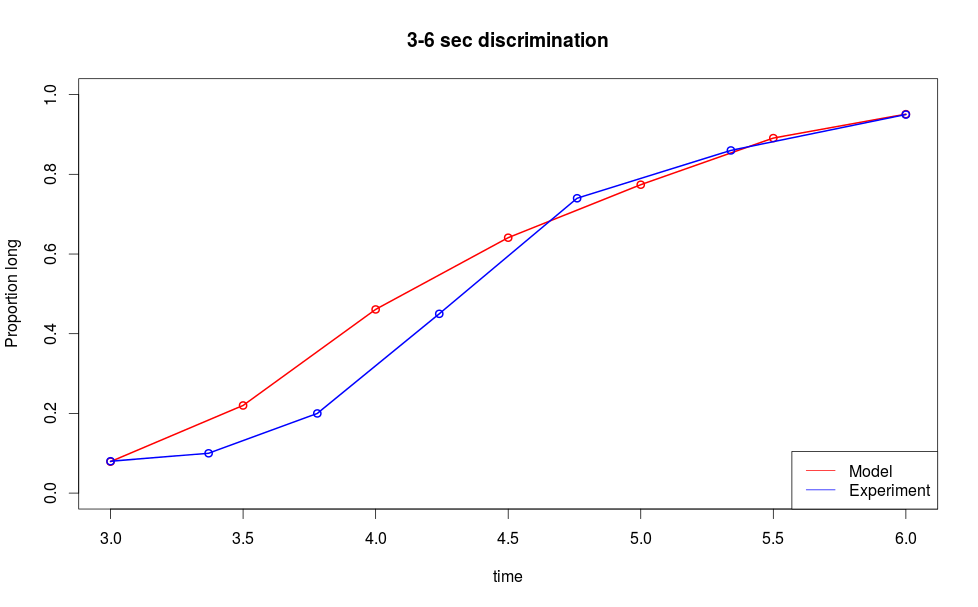
\includegraphics[width=\textwidth]{3-6.png}
\end{figure}
\begin{figure}[H]
\centering
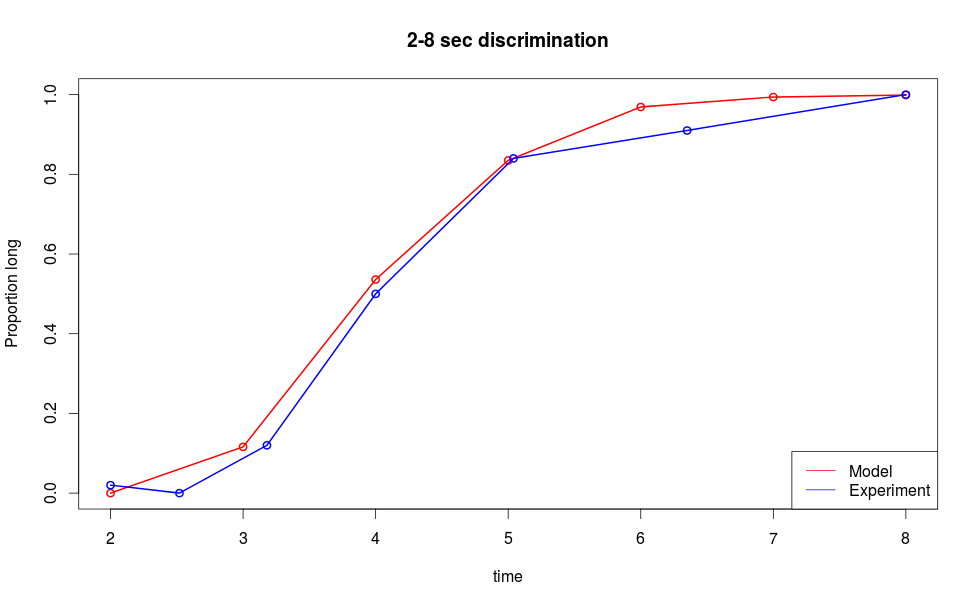
\includegraphics[width=\textwidth]{2-8.png}
\end{figure}
\begin{figure}[H]
\centering
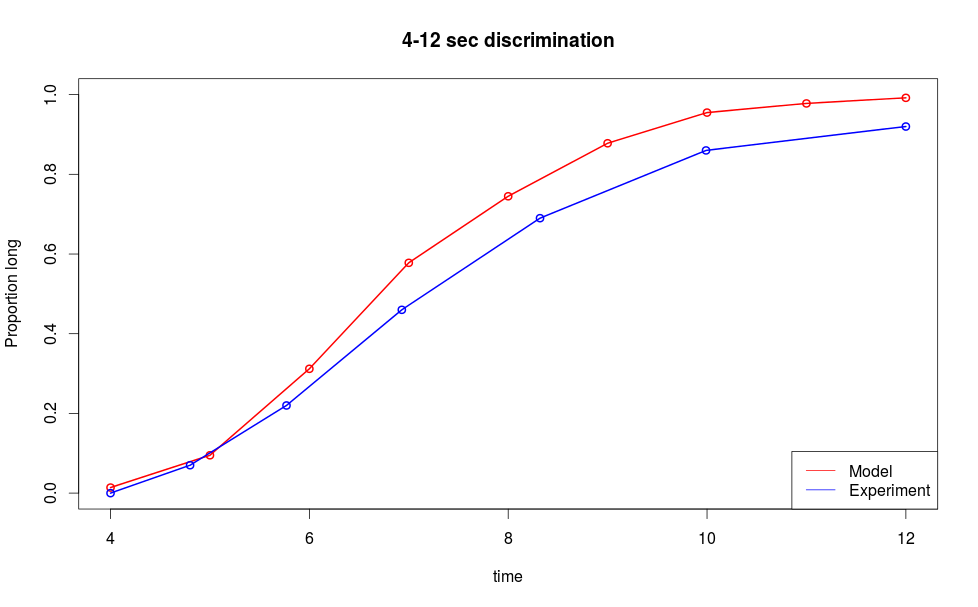
\includegraphics[width=\textwidth]{4-12.png}
\end{figure}


\end{document}
